\documentclass[UTF8]{ctexart}
\usepackage{geometry, CJKutf8}
\geometry{margin=1.5cm, vmargin={0pt,1cm}}
\setlength{\topmargin}{-1.64723cm} % 调整 topmargin
\setlength{\headheight}{12.64723pt} % 设置 headheight
\setlength{\paperheight}{29.7cm}
\setlength{\textheight}{25.3cm}

% useful packages.
\usepackage{amsfonts}
\usepackage{listingsutf8}
\usepackage{amsmath}
\usepackage{amssymb}
\usepackage{amsthm}
\usepackage{enumerate}
\usepackage{graphicx}
\usepackage{multicol}
\usepackage{fancyhdr}
\usepackage{layout}
\usepackage{listings}
\usepackage{float, caption}
\usepackage{fontspec}
\setmonofont{Noto Sans Mono}

\lstset{
    basicstyle=\ttfamily, basewidth=0.5em, inputencoding=utf8, showstringspaces=false, showspaces=false
}

% some common command
\newcommand{\dif}{\mathrm{d}}
\newcommand{\avg}[1]{\left\langle #1 \right\rangle}
\newcommand{\difFrac}[2]{\frac{\dif #1}{\dif #2}}
\newcommand{\pdfFrac}[2]{\frac{\partial #1}{\partial #2}}
\newcommand{\OFL}{\mathrm{OFL}}
\newcommand{\UFL}{\mathrm{UFL}}
\newcommand{\fl}{\mathrm{fl}}
\newcommand{\op}{\odot}
\newcommand{\Eabs}{E_{\mathrm{abs}}}
\newcommand{\Erel}{E_{\mathrm{rel}}}

\begin{document}

\pagestyle{fancy}
\fancyhead{}
\lhead{黎学圣, 3230102179}
\chead{布谷鸟哈希项目}
\rhead{Dec.4th, 2024}

\section{布谷鸟哈希表核心代码}

\subsection{辅助函数:生成素数}
\begin{lstlisting}[language=C++]
auto nextPrime(int n) -> int
{
    if (n <= 2)
        return 2;
    if (n % 2 == 0)
        ++n; // 如果是偶数,先加1变成奇数

    while (true)
    {
        bool isPrime = true;
        int sqrt_n = static_cast<int>(std::sqrt(n));
        for (int i = 3; i <= sqrt_n; i += 2)
        {
            if (n % i == 0)
            {
                isPrime = false;
                break;
            }
        }
        if (isPrime)
        {
            return n;
        }
        n += 2; // 只检查奇数
    }
}
\end{lstlisting}
生成大于等于 \texttt{n} 的下一个素数。素数在哈希表中用于减少冲突。
使用了C++20的auto返回值类型推导。

\subsection{定义可哈希概念}
\begin{lstlisting}[language=C++]
template <typename T>
concept Hashable = requires(T t) {
    { std::hash<T>{}(t) } -> std::convertible_to<std::size_t>;
    { t == t } -> std::convertible_to<bool>;
};
\end{lstlisting}
\texttt{Hashable} 概念确保类型 \texttt{T} 可以被哈希并且支持相等比较。

\subsection{定义可打印概念}
\begin{lstlisting}[language=C++]
template <typename T>
concept Printable = requires(T t, std::ostream &os) {
    { os << t } -> std::convertible_to<std::ostream &>;
};
\end{lstlisting}
\texttt{Printable} 概念确保类型 \texttt{T} 可以被输出到流中。

\subsection{哈希函数族类}
\begin{lstlisting}[language=C++]
template <Hashable Key, typename Hash = std::hash<Key>>
class HashFunctionFamily
{
    std::vector<int> primes;
    int num_functions;
    Hash user_hash;

public:
    explicit HashFunctionFamily(const int num_functions) : num_functions(num_functions)
    {
        if (num_functions <= 0)
        {
            throw std::invalid_argument("Number of hash functions must be positive.");
        }

        for (int i = 0; i < num_functions; ++i)
        {
            primes.push_back(nextPrime(i + 1));
        }
    }

    auto hash(const Key &key, const int function_index, int table_size) const -> int
    {
        return (user_hash(key) + primes[function_index]) % table_size;
    }
};
\end{lstlisting}
这个类生成多个哈希函数,每个函数使用不同的素数来减少冲突。

\subsection{哈希表参数结构体}
\begin{lstlisting}[language=C++]
struct HashTableParams
{
    int initial_table_size = 47;
    double max_load_factor = 0.5;
    int max_rehash_attempts = 50;

    HashTableParams() = default;

    HashTableParams(int initial_table_size,
                    double max_load_factor,
                    int max_rehash_attempts)
    {
        this->initial_table_size = initial_table_size;
        this->max_load_factor = max_load_factor;
        this->max_rehash_attempts = max_rehash_attempts;
    }

    HashTableParams(const HashTableParams &other)
    {
        initial_table_size = other.initial_table_size;
        max_load_factor = other.max_load_factor;
        max_rehash_attempts = other.max_rehash_attempts;
    }

    HashTableParams &operator=(const HashTableParams &other)
    {
        if (this != &other)
        {
            initial_table_size = other.initial_table_size;
            max_load_factor = other.max_load_factor;
            max_rehash_attempts = other.max_rehash_attempts;
        }
        return *this;
    }
};

static HashTableParams hashTableParams;
\end{lstlisting}
这个结构体定义了哈希表的参数,并提供了默认构造函数、复制构造函数和赋值运算符。
哈希表的三个参数分别为初始表大小、最大负载因子和最大重新哈希尝试次数。

\subsection{布谷鸟哈希表类}
\begin{lstlisting}[language=C++]
template <Hashable Key, typename Hash = std::hash<Key>>
class CuckooHashTable
{
    int INITIAL_TABLE_SIZE = hashTableParams.initial_table_size;
    double MAX_LOAD_FACTOR = hashTableParams.max_load_factor;
    int MAX_REHASH_ATTEMPTS = hashTableParams.max_rehash_attempts;

    std::vector<std::vector<std::optional<Key>>> tables; // 多张哈希表
    int num_elements;                                    // 元素个数
    int table_size;                                      // 当前哈希表大小
    HashFunctionFamily<Key, Hash> hash_functions;

    void rehash();
    auto loadFactor() const -> double;

public:
    explicit CuckooHashTable(const int num_functions);
    void insert(const Key &key);
    void insert(Key &&key);
    auto find(const Key &key) const -> bool;
    void erase(const Key &key);
    void printTable() const requires Printable<Key>;
};
\end{lstlisting}
这个类实现了布谷鸟哈希表的主要功能,包括插入、查找、删除和重新哈希。
哈希表参数从结构体中获取,哈希函数族类用于生成多个哈希函数。
这里的模板确保元素类型是可哈希的,用户自定义类必须实现哈希函数和相等比较,
这有点像Java中的接口,但是C++的模板更加灵活。
C++的标准库类如int、string等显然都满足概念约束。

\subsubsection{构造函数}
\begin{lstlisting}[language=C++]
explicit CuckooHashTable(const int num_functions) : num_elements(0), table_size(INITIAL_TABLE_SIZE),
                                                    hash_functions(num_functions)
{
    tables.assign(num_functions, std::vector<std::optional<Key>>(table_size));
}
\end{lstlisting}
构造函数初始化哈希表的参数,并分配多张哈希表。
\texttt{std::optional} 的意思是这个位置可能为空,
这样可以区分空位置和有值的位置。这就跟Rust的Option类似。

\subsubsection{重新哈希函数}
\begin{lstlisting}[language=C++]
void rehash()
{
    std::cout << "Rehashing..." << std::endl;
    auto old_tables = tables;                                                  // 保存旧表
    table_size = nextPrime(2 * table_size);                                    // 扩大表
    tables.assign(tables.size(), std::vector<std::optional<Key>>(table_size)); // 重新分配表

    num_elements = 0;

    // 重新插入元素
    for (const auto &old_table : old_tables)
    {
        for (const auto &key : old_table)
        {
            if (key.has_value())
            {
                insert(std::move(key.value()));
            }
        }
    }
}
\end{lstlisting}
重新哈希函数在负载因子超过最大值或插入失败时重新分配表并重新插入元素。
先备份旧表,然后扩大表(大小为两倍大小的下一个素数),
然后重新分配表,然后重新插入元素。

\subsubsection{计算负载因子函数}
\begin{lstlisting}[language=C++]
auto loadFactor() const -> double
{
    return static_cast<double>(num_elements) / (tables.size() * table_size);
}
\end{lstlisting}
计算负载因子,用于判断是否需要重新哈希。

\subsubsection{插入元素函数(左值引用)}
\begin{lstlisting}[language=C++]
void insert(const Key &key)
{
    Key temp_key = key;
    insert(std::move(temp_key));
}
\end{lstlisting}
插入元素(左值引用),调用右值引用版本的插入函数。
这样可以少写一些代码,提高代码复用性。

\subsubsection{插入元素函数(右值引用)}
\begin{lstlisting}[language=C++]
void insert(Key &&key)
{
    if (loadFactor() > MAX_LOAD_FACTOR)
    {
        rehash();
    }

    int attempts = 0;
    std::random_device rd;
    std::mt19937 gen(rd());
    std::uniform_int_distribution<> table_dist(0, tables.size() - 1);

    while (attempts < MAX_REHASH_ATTEMPTS)
    {
        for (int i = 0; i < tables.size(); ++i)
        {
            int index = hash_functions.hash(key, i, table_size);
            if (!tables[i][index].has_value())
            {
                tables[i][index] = std::move(key);
                ++num_elements;
                return;
            }
            // 替换已有元素
            std::swap(key, tables[i][index].value());
        }

        // 没有可用位置,随机踢出一个元素
        int table_index = table_dist(gen);
        int index = hash_functions.hash(key, table_index, table_size);
        std::swap(key, tables[table_index][index].value());
        ++attempts;
    }

    // 超过最大次数
    rehash();
    insert(std::move(key));
}
\end{lstlisting}
插入元素(右值引用)是布谷鸟哈希表的核心功能之一。该函数的主要任务是将一个元素插入到哈希表中,并在必要时进行重新哈希。

首先,函数检查当前的负载因子(即表中已使用的槽位与总槽位的比例)。如果负载因子超过了预设的最大值,则调用 \texttt{rehash()} 函数进行重新哈希,以扩大哈希表的容量。

接下来,函数初始化一个随机数生成器 \texttt{std::random\_device} 和一个梅森旋转算法引擎 \texttt{std::mt19937},用于在插入过程中随机选择表和槽位。

函数进入一个循环,最多尝试 \texttt{MAX\_REHASH\_ATTEMPTS} 次插入操作。
在每次尝试中,函数遍历所有的哈希表,并计算元素在每个表中的哈希值。
如果找到一个空槽(即 \texttt{std::optional} 没有值),
则将元素插入该槽,并增加元素计数 \texttt{num\_elements},然后返回。

如果所有的槽位都已被占用,函数会随机选择一个表和槽位,将当前元素与该槽位中的元素交换,并继续尝试插入交换后的元素。

如果在最大尝试次数内仍未能成功插入元素,函数会调用 \texttt{rehash()} 函数进行重新哈希,然后再次尝试插入元素。

这种插入策略确保了哈希表在高负载情况下仍能高效地插入元素,同时通过重新哈希和随机踢出策略来减少冲突。

\subsubsection{查找元素函数}
\begin{lstlisting}[language=C++]
auto find(const Key &key) const -> bool
{
    for (int i = 0; i < tables.size(); ++i)
    {
        int index = hash_functions.hash(key, i, table_size);
        if (tables[i][index].has_value() && tables[i][index].value() == key)
        {
            return true;
        }
    }

    return false;
}
\end{lstlisting}
查找元素,返回元素是否存在。核心是遍历哈希函数族生成的哈希值,查找元素是否存在。

\subsubsection{删除元素函数}
\begin{lstlisting}[language=C++]
void erase(const Key &key)
{
    for (int i = 0; i < tables.size(); ++i)
    {
        int index = hash_functions.hash(key, i, table_size);
        if (tables[i][index].has_value() && tables[i][index].value() == key)
        {
            tables[i][index].reset();
            --num_elements;
            return;
        }
    }

    throw std::runtime_error("Key not found.");
}
\end{lstlisting}
删除元素,如果元素存在则删除,否则抛出异常。
删除元素是使用 \texttt{std::optional} 的 \texttt{reset()} 函数
来实现的,将槽位重置为空。

\subsubsection{打印哈希表函数}
\begin{lstlisting}[language=C++]
void printTable() const
    requires Printable<Key>
{
    for (int i = 0; i < tables.size(); ++i)
    {
        std::cout << "Table " << i << ": ";
        for (int j = 0; j < table_size; ++j)
        {
            if (tables[i][j].has_value())
            {
                std::cout << tables[i][j].value() << " ";
            }
            else
            {
                std::cout << "- ";
            }
        }
        std::cout << std::endl;
    }
}
\end{lstlisting}
打印哈希表的状态,要求元素类型实现 \texttt{Printable} 概念。

\section{布谷鸟哈希测试}

\subsection{测试代码}
\begin{lstlisting}[language=C++]
#include <iostream>
#include <vector>
#include <chrono>
#include <fstream>
#include <random>
#include "cuckoo.h"
#include "student.h"

int main()
{
    std::vector<int> data_sizes;
    for (int i = 1000; i <= 20000; i += 100)
    {
        data_sizes.push_back(i);
    }
    constexpr int num_hash_functions = 20;

    std::ofstream insert_outfile("insert_times.txt");
    std::ofstream search_outfile("search_times.txt");
    if (!insert_outfile.is_open() || !search_outfile.is_open())
    {
        std::cerr << "Failed to open file for writing.\n";
        return 1;
    }

    std::random_device rd;
    std::mt19937 gen(rd());

    for (const auto &num_students : data_sizes)
    {
        std::vector<Student> students;
        for (int i = 1; i <= num_students; ++i)
        {
            students.emplace_back("Stu" + std::to_string(i), "Tom" + std::to_string(i));
        }

        // INITIAL_TABLE_SIZE, MAX_LOAD_FACTOR, MAX_REHASH_ATTEMPTS
        hashTableParams = HashTableParams(203, 0.45, 100);

        // 测试插入性能
        {
            CuckooHashTable<Student> cuckoo_table(num_hash_functions);
            auto start_time = std::chrono::high_resolution_clock::now();
            for (const auto &student : students)
            {
                cuckoo_table.insert(student);
            }
            auto end_time = std::chrono::high_resolution_clock::now();
            std::chrono::duration<double> duration = end_time - start_time;
            insert_outfile << num_students << " " << duration.count() << "\n";
            std::cout << "Inserted " << num_students << " students in " << duration.count() << " seconds.\n";

            // 测试查找性能
            std::uniform_int_distribution<> dis(0, num_students - 1);
            int random_index = dis(gen);
            const auto &random_student = students[random_index];

            start_time = std::chrono::high_resolution_clock::now();
            cuckoo_table.find(random_student);
            end_time = std::chrono::high_resolution_clock::now();
            duration = end_time - start_time;
            search_outfile << num_students << " " << duration.count() << "\n";
            std::cout << "Searched for student " << random_student.id << " in " << duration.count() << " seconds.\n";
        }
    }

    insert_outfile.close();
    search_outfile.close();
    return 0;
}
\end{lstlisting}

\subsection{测试说明}
在这段代码中,我们测试了布谷鸟哈希表的插入和查找性能。具体步骤如下:

\begin{enumerate}
    \item 初始化数据集规模,从 1000 到 20000,每次增加 100。
    \item 定义哈希函数的数量为 20。
    \item 打开两个输出文件,分别用于记录插入时间和查找时间。
    \item 使用随机数生成器生成随机数据。
    \item 对于每个数据集规模:
    \begin{enumerate}
        \item 生成对应数量的学生数据。
        \item 设置哈希表参数,包括初始表大小、最大负载因子和最大重新哈希尝试次数。
        \item 测试插入性能:
        \begin{enumerate}
            \item 创建布谷鸟哈希表。
            \item 记录插入开始时间。
            \item 插入所有学生数据。
            \item 记录插入结束时间。
            \item 计算插入时间并写入文件。
        \end{enumerate}
        \item 测试查找性能:
        \begin{enumerate}
            \item 随机选择一个学生。
            \item 记录查找开始时间。
            \item 查找该学生。
            \item 记录查找结束时间。
            \item 计算查找时间并写入文件。
        \end{enumerate}
    \end{enumerate}
    \item 关闭输出文件。
\end{enumerate}

通过这些测试,我们可以评估布谷鸟哈希表在不同数据集规模下的插入和查找性能,并将结果记录到文件中以便进一步分析。

\section{测试图像}

在本节中,我们展示了布谷鸟哈希表的插入和查找时间复杂度的测试结果图像。

\subsection{插入时间复杂度}
\begin{figure}[H]
    \centering
    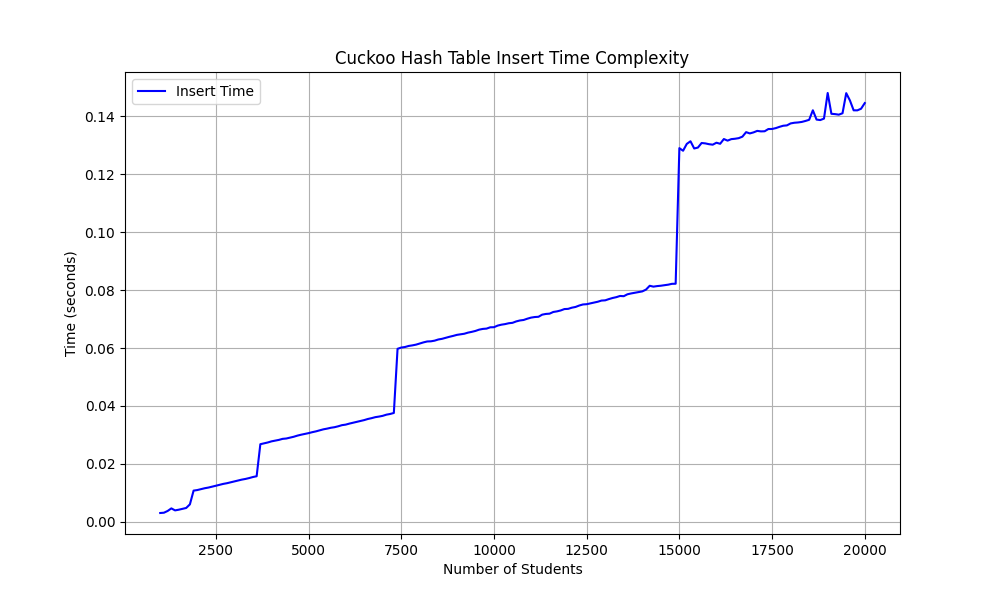
\includegraphics[width=0.8\textwidth]{insert_times.png}
    \caption{Cuckoo Hash Table Insert Time Complexity}
    \label{fig:insert_times}
\end{figure}

从图中可以看出,随着学生数量的增加,插入时间总体上呈现出上升的趋势。
在某些点上,插入时间有明显的跳跃,这表示发生了重新哈希(rehashing)
的操作。

在两个跳跃之间的斜线部分,插入时间相对稳定且逐渐增加。
这些斜线部分表明,在两次重新哈希之间,随着学生数量的增加,
插入操作的时间也在逐渐增加,但增长较为平缓。
这种趋势反映了布谷鸟哈希表在未达到重新哈希阈值时的正常工作状态,
即随着负载的增加,插入时间线性增长,但总体上仍然保持高效。

\subsection{查找时间复杂度}
\begin{figure}[H]
    \centering
    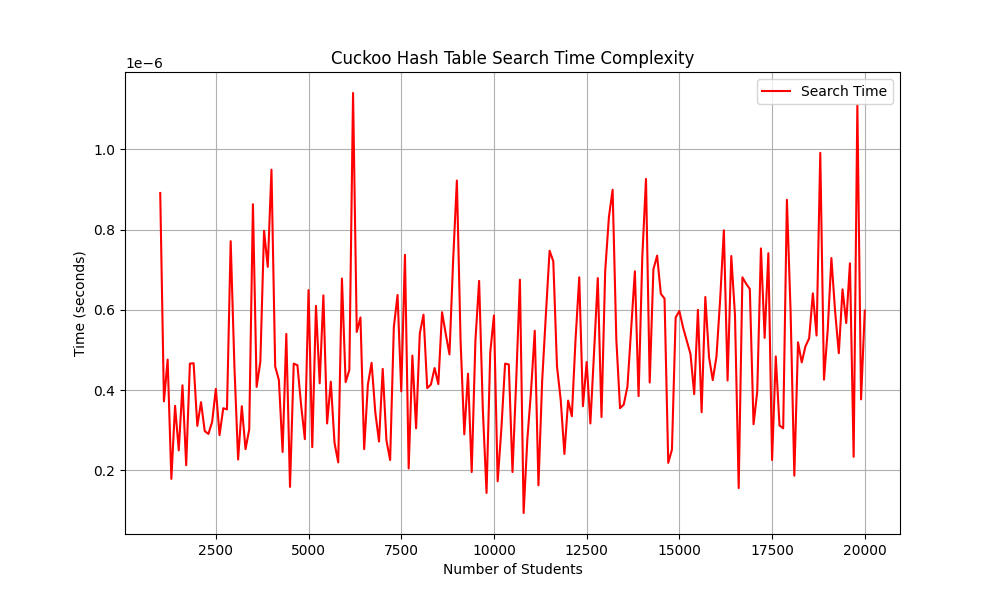
\includegraphics[width=0.8\textwidth]{search_times.png}
    \caption{Cuckoo Hash Table Search Time Complexity}
    \label{fig:search_times}
\end{figure}

从图中可以看出,搜索时间呈现出明显的波动。
总体来看,搜索时间在不同学生数量下波动较大,
但总体趋势并不明显,显示出布谷鸟哈希表在搜索操作上的随机性和不确定性。

在两个显著峰值之间的斜线部分,搜索时间的波动较为频繁,
但总体上保持在较低的范围内。这些斜线部分表明,在两次显著峰值之间,
搜索时间虽然有波动,但总体上仍然保持在较低的水平,
显示出布谷鸟哈希表在搜索操作上的高效性和稳定性。

\subsection{运行测试}
要运行测试并生成图像,请使用以下命令:

\begin{verbatim}
make
make test
\end{verbatim}

\noindent 该命令将执行以下步骤:
\begin{enumerate}
    \item 编译并运行 \texttt{main.cpp},生成插入和查找时间数据文件 \texttt{insert\_times.txt} 和 \texttt{search\_times.txt}。
    \item 使用 Python 脚本 \texttt{test.py} 读取数据文件并生成图像。
\end{enumerate}

\noindent 以下是 \texttt{Makefile} 中的相关部分:

\begin{verbatim}
test:
    ./main
    python3 test.py
\end{verbatim}

通过运行 \texttt{make test},可以生成并查看布谷鸟哈希表的插入和查找时间复杂度图像。

\end{document}
